\chapter{Aufgabenstellung und Zielformulierung}

\section{Ausgangslage}

Wie bereits erw�hnt, mangelt es momentan in der Medienwelt nicht an Begeisterung f�r Virtual Reality. In Foren wird dar�ber diskutiert, an Events wird es demonstriert und t�glich finden neue Infos ihren Weg in die �ffentlichkeit.

Ein wesentliches Problem ist allerdings die Eingabe. Gl�cklicherweise gibt es bereits zu einem erschwinglichen Preis eine M�glichkeit, die eigenen zwei H�nde zu verwenden und zu erkennen: die Leap Motion.

Sie ist zu einem Preis von \EUR{89.99} erh�ltlich und erm�glicht eine rein visuelle Handerkennung ohne Handschuhe oder �hnlichen Zusatz.

\begin{figure}[h]
	\centering
	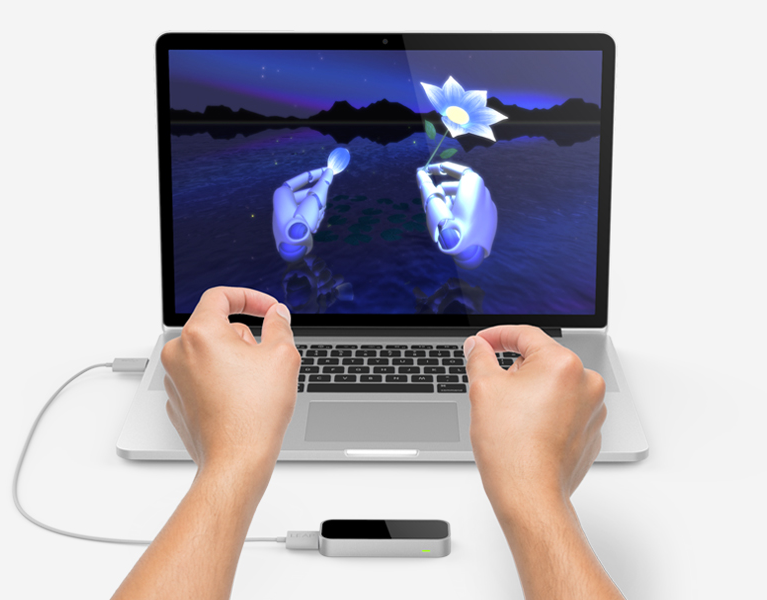
\includegraphics[width=0.5\linewidth]{bilder/leap_example}
	\caption{Die Leap Motion im Einsatz}
	\source{https://www.leapmotion.com/}
	\label{fig:leap_example}
\end{figure}

Im Vorprojekt, das ebenfalls bereits erw�hnt wurde, stellte sich aus, dass jedoch Vorsicht beim Einsatz der Leap Motion geboten ist. Die Erkennung ist nicht stabil und gewisse Positionen funktionieren besser als andere. Es stellten sich also ein paar Anforderungen an eine Einbindung:

\begin{itemize}
	\item Die Applikation darf nicht auf schnelle und genaue Eingabe des Benutzers basieren
	\item Gesten m�ssen mit Bedacht des Sichtfeldes konzipiert werden
\end{itemize}

Besonders der erste Punkt schliesst eine Anwendung der Leap Motion in einem Spiel aus. Bei einem Spiel w�rden die H�nde unausweichlich in den Vordergrund des Spielkonzeptes r�cken und eine essenzielle Rolle �bernehmen. Da allerdings die Handerkennung nicht zuverl�ssig ist, geschehen Fehler. Unbeabsichtigte Operationen passieren, der Spieler verliert, er ist frustriert und nach kurzer Zeit gibt er das Spiel auf.

Der gew�hlte Ansatz ist jedoch ein anderer: Kein Spiel soll erstellt werden, sondern eine Applikation, die durch die H�nde gesteuert werden kann und dadurch einen speziellen Charme erh�lt. Es folgt die Zielformulierung.


\section{Urspr�ngliche Zielformulierung}

Es soll eine Applikation namens ``\gls{imvr}'' entwickelt werden, welche Gebrauch von der Oculus Rift macht, um die Bild- und Musiksammlung des Anwenders ansprechend darzustellen, z.B. in Form eines 3D-Karussels. Die zus�tzliche "Tiefe", die durch den Einsatz eines stereoskopischen \gls{hmd} entsteht, soll dem Anwender helfen, sich in seiner Medienbibliothek schneller zurechtzufinden.

Zus�tzlich dazu soll die Leap Motion dazu verwendet werden, um vollst�ndige Handfreiheit zu gew�hren: Der Anwender soll komplett ohne Maus und Tastatur imstande sein, sich durch seine Bilder zu navigieren.

Kurz zusammengefasst muss die Applikation:

\begin{itemize}
	\item Die Bilder- und Musikbibliothek des Benutzers in stereoskopischem 3D darstellen.
	\item Diese freih�ndig durchsuchbar machen mit Sortier- und evtl. Gruppierfunktion.
	\item Die Bilder betrachtbar und die Musik abspielbar machen.
	\item Metainformationen darstellen (z.B. in Form von Diagrammen).
\end{itemize}

Zus�tzlich zur Applikation selbst soll noch ein zus�tzliches Tool entwickelt werden, welches im Voraus die Dateien auf dem Host-System indexiert und f�r die visuelle Applikation bereitstellt.

\section{�nderungen an der Zielformulierung}

Aufgrund der begrenzten Zeit und eines vermehrten Interesse in die Darstellung von Musik, wurde die Zielformulierung w�hrend des Projekts leicht abge�ndert:

\begin{itemize}
	\item Die Bilderbibliothek f�llt weg
	\item Die Sortier- und Gruppierfunktion f�llt weg
	\item Es wird mehr Gewicht auf die Darstellungsweise der Musik gelegt
\end{itemize}

Dazu ist zu sagen, dass auch weiterhin stark auf Bildervisualisierung gesetzt wird. Anstatt den Computer des Anwenders auf Bilder abzuscannen wird diese jedoch vollst�ndig um die lokale Musik aufgebaut. Konkret bedeutet das, dass Artwork von Alben und Fotos von Artisten dargestellt wird.

Die im zweiten Punkt erw�hnte Sortier- und Gruppierfunktion k�nnte in einem weiteren Schritt nachgereicht werden, wurde aber im momentanen Stadium zugunsten von anderen Features vernachl�ssigt.

\section{Hilfsmittel \& Hardware}

Verschieden Hilfsmittel werden f�r die Durchf�hrung des Projektes gebraucht. Seitens Software lauten diese:

\begin{table}[H]
	\caption{�bersicht der eingesetzten Software}
	\centering
	\label{tab:software}
	\begin{tabular}{ l l l }
		\noalign{\smallskip} \hline \hline \noalign{\smallskip}
		\textbf{Name} & \textbf{Beschreibung} \\ \midrule
		Unity3D & Spielengine und Entwicklungsumgebung \\
		Visual Studio 2012 \& 2013 & Entwicklungsumgebung von Microsoft \\
		Blender & Open-Source 3D Modelling-Tool \\
		Krita & Open-Source Grafikbearbeitungs-Tool \\
		GIMP & Open-Source Grafikbearbeitungs-Tool \\
		LaTeX & Hilfsmittel f�r die Erstellung wissenschaftlicher Dokumente \\
		Microsoft Visio & Tool zur Erstellung von Diagrammen \\
		\noalign{\smallskip} \hline \noalign{\smallskip}
	\end{tabular}
\end{table}

Im Hardware-Departement wurde folgendes eingesetzt:

\begin{table}[H]
	\caption{�bersicht der eingesetzten Hardware}
	\centering
	\label{tab:hardware}
	\begin{tabular}{ l l l }
		\noalign{\smallskip} \hline \hline \noalign{\smallskip}
		\textbf{Name} & \textbf{Beschreibung} \\ \midrule
		Oculus Rift & \gls{hmd} von Oculus VR \\
		Leap Motion & Hand- und Fingererkennungsger�t von Leap Motion, Inc. \\
		\noalign{\smallskip} \hline \noalign{\smallskip}
	\end{tabular}
\end{table}

F�r eine genaue Erkl�rung der Oculus Rift und der Leap Motion sei an dieser Stelle auf das Pflichtenheft und die Vorarbeit verwiesen, welche diese im Detail einf�hrt.